\documentclass[12pt]{article}

\usepackage[hmargin=.65in, vmargin=.7in]{geometry}
\usepackage[citecolor=blue, colorlinks=true, linkcolor=blue, urlcolor=blue]{hyperref}
\usepackage{natbib}
\usepackage{graphicx}
\usepackage{multirow}
\usepackage{tabularx}
\usepackage[table, svgnames]{xcolor}
\usepackage{authblk}
\usepackage{booktabs}
\usepackage[toc,page]{appendix}
\usepackage[T1]{fontenc}
\usepackage{enumitem}
\usepackage{caption}
\usepackage{array}

\title{A Standard for Exchangeable Magnetotelluric Metadata}
\date{\textbf{Version 0.0.15 -- June 2020}\footnote{\noindent\textbf{\textit{Corresponding Authors:}}
		
		Jared Peacock (\url{jpeacock@usgs.gov})
		
		Andy Frassetto (\url{andy.frassetto@iris.edu})}}
\author[1]{Working Group for Data Handling and Software - PASSCAL Magnetotelluric Program}
\affil[1]{Portable Array Seismic Studies of the Continental Lithosphere, Incorporated Research Institutions for Seismology}

\newcommand{\attr}[1]{\textbf{#1}}
\newcommand{\True}[0]{{\color{Red}{\textbf{True}}}}
\newcommand{\False}[0]{{\color{Teal}{\textbf{False}}}}

\renewcommand{\arraystretch}{1.0}

\newcommand{\entry}[7]{
	\textbf{#1} 
	\begin{itemize}[topsep=5pt,itemsep=-.1pt,parsep=-2pt,partopsep=0pt,labelwidth=2em,align=left,itemindent=1em]
		\begin{small}
			\item[Required:] #2
			\item[Units:] #3
			\item[Type:] #4
			\item[Style:] #5
		\end{small}
	\end{itemize} & #6 & #7 \\ \midrule}

\begin{document}
	
\maketitle

\clearpage
\newpage
\tableofcontents
\addcontentsline{toc}{section}{\listtablename}
\listoftables
\vspace{1cm}

\rowcolors{1}{white}{AliceBlue}

\newpage

\section{Introduction}

Researchers using magnetotelluric (MT) methods lack a standardized format for storing time series data and metadata. Commercially available MT instruments produce data in formats that range from proprietary binary to ASCII, whereas recent datasets from the U.S. MT community have utilized institutional formats or heavily adapted formats like miniSEED. In many cases, the available metadata for MT time series are incomplete and loosely standardized; and overall, these datasets are not "user friendly". This lack of a standardized resource impedes the exchange and broader use of these data beyond a small community of specialists.

The \href{https://www.iris.edu/hq/programs/passcal/magnetotelluricnstrumentation}{IRIS PASSCAL MT facility} maintains a pool of MT instruments that are freely available to U.S. Principal Investigators (PIs). Datasets collected with these instruments are subject to data sharing requirements, and an IRIS \href{https://www.iris.edu/hq/aboutris/governance/mtoft}{working group} advises the development of sustainable data formats and workflows for this facility. Following in the spirit of the standard created for \href{https://library.seg.org/doi/10.1190/geo2018-0679.1}{MT transfer function} datasets, this document outlines a new metadata standard for level 0,1,and 2 MT time series data (\href{https://earthdata.nasa.gov/collaborate/open-data-services-and-software/data-information-policy/data-levels}{Data Levels}). Following community approval of these standards, MTH5 (an HDF5 MT specific format) will be developed later in 2020.

The Python 3 module written for these standards and MTH5 is being developed at \url{https://github.com/kujaku11/MTarchive/tree/tables}.

\section{General Structure}

The metadata for a full MT dataset are structured to cover details from single channel time series to a full survey. For simplicity, each of the different scales of an MT survey and measurements have been categorized starting from largest to smallest (Figure \ref{fig:example}). These categories are: \verb|Survey|, \verb|Station|, \verb|Run|, \verb|DataLogger|, \verb|Electric Channel|, \verb|Magnetic Channel|, and \verb|Auxiliary Channel|. Each category is described in subsequent sections.  Required keywords are labeled as \True\quad and suggested keywords are labeled as \False. A user should use as much of the suggested metadata as possible for a full description of the data.  

\begin{figure}[htb!]
	\centering
	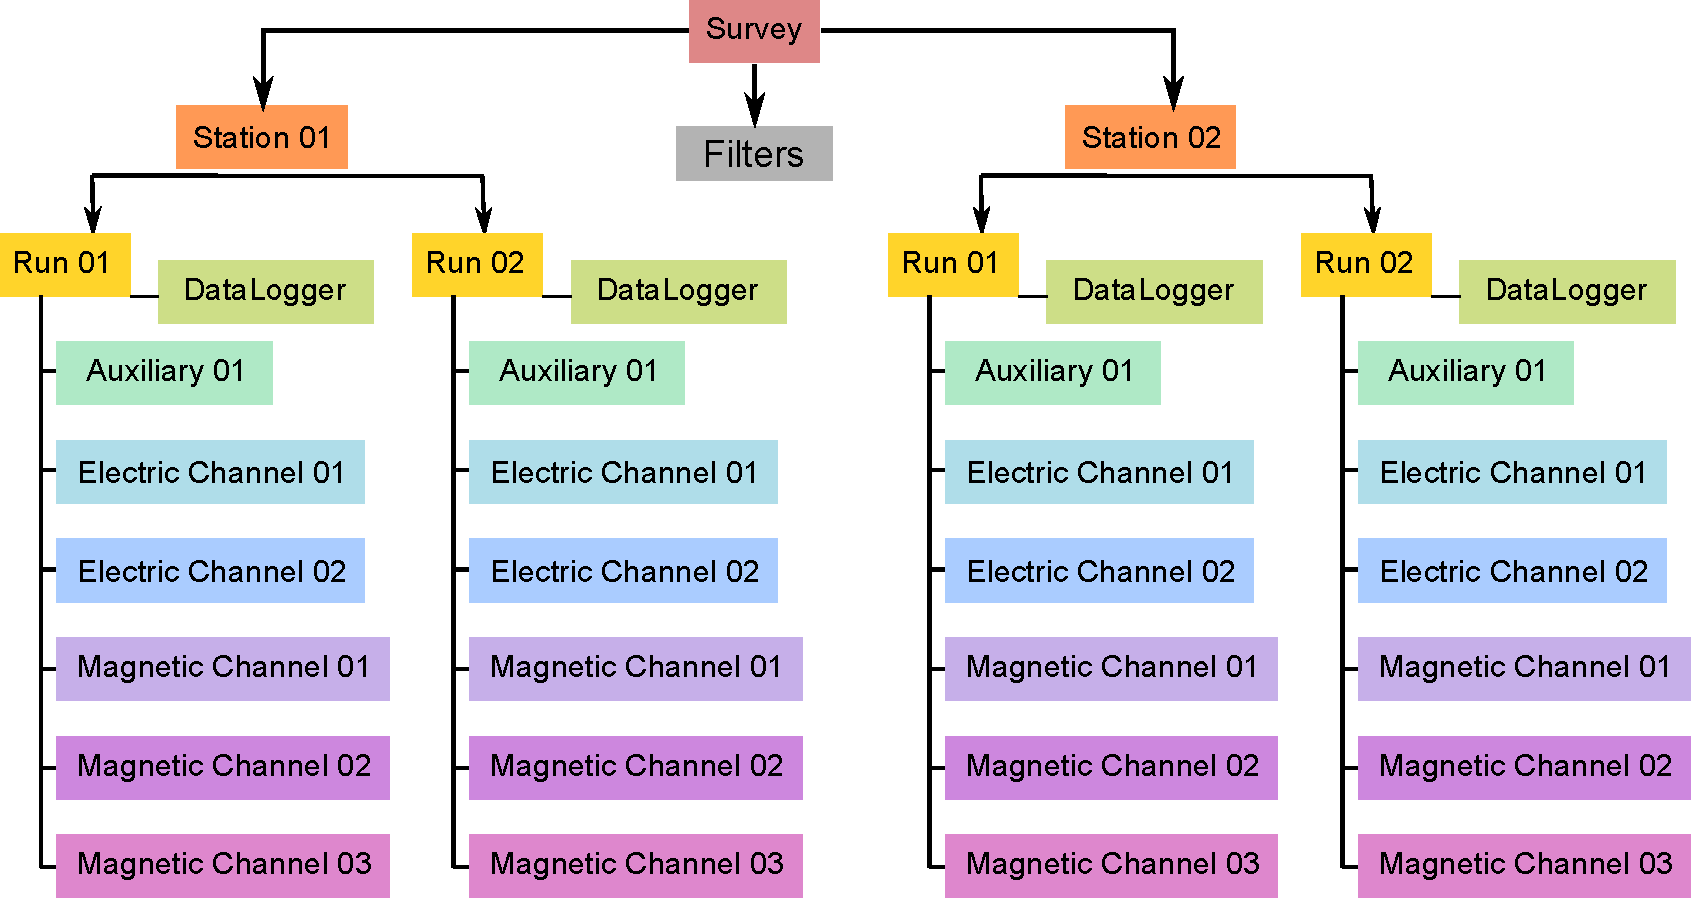
\includegraphics[height=.525\textwidth]{example_mt_file_structure.pdf}
	\caption{Schematic of a MT time series file structure with appropriate metadata. The top level is the \textit{Survey} that contains general information about who, what, when, where, and how the data were collected.  Underneath \textit{Survey} are the \textit{Station} and \textit{Filter}.  \textit{Filter} contains information about different filters that need to be applied to the raw data to get appropriate units and calibrated measurements.  Underneath \textit{Station} are \textit{Run}, which contain data that were collected at a single sampling rate with common start and end time. Finally, \textit{Channel} describes each channel of data collected and can be an \textit{Auxiliary}, \textit{Electric}, or \textit{Magnetic}.  Metadata is attributed based on the type of data collected in the channel.}
	\label{fig:example}
\end{figure}

\subsection{Metadata Keyword Format}

The metadata key names should be self-explanatory and are structured as follows:\\ \verb|{category}.{name}|, where:
\begin{itemize}
	\item \verb|category| refers to a metadata category or level that has common parameters, such as \verb|location|, which will have a latitude, longitude, and elevation $\longrightarrow$ \verb|location.latitude|, \verb|location.longitude|, and \verb|location.elevation|.  These can be nested, for example, \verb|positive.location.latitude|
	\item \verb|name| is a descriptive name, where words should be separated by an underscore. Note that only whole words should be used and abbreviations should be avoided, e.g. \verb|data_quality|.  
\end{itemize}  

A '.' represents the separator between different categories.  The metadata can be stored in many different forms.  Common forms are XML or JSON formats.  See examples below for various ways to represent the metadata.      

\subsection{Formatting Standards}

Specific and required formatting standards for location, time and date, and angles are defined below and should be adhered to.

\subsubsection{Time and Date Format}

All time and dates are given as an ISO formatted date-time String in the UTC time zone.  The ISO Date Time format is \verb|YYYY-MM-DDThh:mm:ss.ms+00:00|, where the UTC time zone is represented by \verb|+00:00|. If the data requires a different time zone, this can be accommodated but it is recommended that UTC be used whenever possible to avoid confusion of local time and local daylight savings. Milliseconds can be accurate to 6 decimal places.  ISO dates are formatted \verb|YYYY-MM-DD|.  Hours are given as a 24 hour number or military time, e.g. 4:00 PM is 16:00.

\subsubsection{Location}

All latitude and longitude locations are given in decimal degrees in the well known datum specified at the \verb|Survey| level. \textbf{NOTE: The entire survey should use only one datum that is specified at the Survey level.}

\begin{itemize}
	\setlength\itemsep{0em}
	\item All latitude values must be $<|90|$ and all longitude values must be $<|180|$.
	\item Elevation and other distance values are given in meters.
	\item Datum should be one of the well known datums, WGS84 is preferred, but others are acceptable.
\end{itemize} 

\subsubsection{Angles}

All angles of orientation are given in decimal degrees.  Orientation of channels should be given in a geographic or a geomagnetic reference frame where the right-hand coordinates are assumed to be North = 0, East = 90, and vertical is positive downward.  The coordinate reference frame is given at the station level \verb|station.orientation.reference_frame|.  Two angles to describe the orientation of a sensor is given by \verb|channel.measurement_azimuth| and \verb|channel.measurement_tilt|.  In a geographic or geomagnetic reference frame, the azimuth refers to the horizontal angle relative to north positive clockwise, and the tilt refers to the vertical angle with 0 perpendicular downwards.  So a tilt angle of 0 points downward, 90 is parallel with the surface, and 180 points upwards.  

Archived data should remain in measurement coordinates. Any transformation of coordinates for derived products can store the transformation angles at the channel level in \\ \verb|channel.transformed_azimuth| and \verb|channel.transformed_tilt|, the transformed reference frame can then be recorded in \verb|station.orientation.transformed_reference_frame|.      

\begin{figure}[!h]
	\centering
	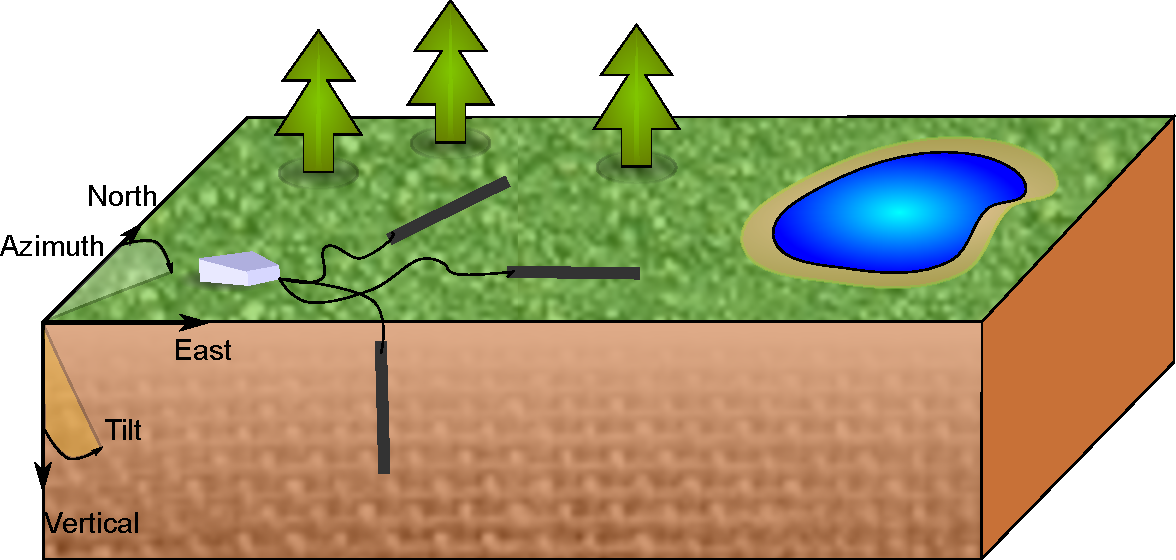
\includegraphics[width=.85\textwidth]{reference_frame.pdf}
	\caption{Diagram showing a right-handed geographic coordinate system.  The azimuth is measured positive clockwise along the horizontal axis and tilt is measured from the vertical axis with postive down = 0, positive up = 180, and horizontal = 90.}
	\label{fig:reference}
\end{figure}  

\subsection{Units}
Acceptable units are only those from the International System of Units (SI).  Only long names in all lower case are acceptable.  Table \ref{tab:units} summarizes common acceptable units.


\begin{table}[!h]
	\centering
	\caption[Acceptable Units]{Acceptable Units}
	\begin{tabular}{ll}
		\toprule
		\textbf{Measurement Type} & \textbf{Unit Name} \\ \midrule
		Angles & decimal degrees \\ \midrule
		
		Distance &  meters  \\ \midrule
		Electric Field & millivolts\\ \midrule
		Latitude/Longitude & decimal degrees \\ \midrule
		Magnetic Field & nanotesla \\ \midrule
		Resistance & ohms   \\ \midrule
		Resistivity & ohm-meters \\ \midrule
		Temperature & celsius\\ \midrule
		Time & seconds\\ \midrule
		Voltage & volts \\ \bottomrule
		
		
	\end{tabular}
	\label{tab:units}
\end{table}

\subsection{String Formats}

Each metadata can have a specific string style, such as date and time or alpha-numeric.  These are described in Table \ref{tab:values}.  Note that any list should be comma separated.

\begin{table}[hb!]
	\centering
	\caption[Acceptable String Formats]{Acceptable String Formats}
	\begin{tabular}{>{\raggedright}p{.9in}>{\raggedright}p{3.2in}c}
		\toprule
		\textbf{Style} & \textbf{Description}  & \textbf{Example} \\ \midrule
		Free Form & An unregulated string that can contain \{a-z, A-Z, 0-9\} and special characters & This is Free Form! \\ \midrule
		
		Alpha Numeric & A string that contains no spaces and only characters \{a-z, A-Z, 0-9, -, /, \_\} & WGS84 or GEOMAG-USGS \\ \midrule
		Controlled Vocabulary & Only certain names or words are allowed. In this case, examples of acceptable values are provided in the documentation as [ option01 $|$ option02 $|$ ...]. The ... indicates that other options are possible but have not been defined yet &  reference\_frame = geographic \\ \midrule
		List & List of entries using a comma separator & Ex, Ey, Hx, Hy, Hz, T' \\ \midrule
		Number & A number according to the data type; number of decimal places has not been implemented yet & 10.0 (float) or 10 (integer) \\ \midrule
		Date & ISO formatted date YYYY-MM-DD in UTC & 2020-02-02 \\ \midrule
		Date Time & ISO formatted date time YYYY-MM-DDThh:mm:ss.ms+00:00 in UTC & 2020-02-02T12:20:45.123456+00:00 \\ \midrule
		Email & A valid email address & \url{person@mt.org} \\ \midrule
		URL & A full URL that a user can view in a web browser  &  \url{https://www.passcal.nmt.edu/} \\ \bottomrule
		
		
	\end{tabular}
	\label{tab:values}
\end{table}

\clearpage
\newpage
\section{Survey}

A survey describes an entire data set that covers a specific time span and region. This may include multiple PIs in multiple data collection episodes but should be confined to a specific experiment or project. The \verb|Survey| metadata category describes the general parameters of the survey.

\begin{table}[h!]
	\caption[Attributes for Survey]{Attributes for Survey }
	\begin{tabular}{p{.275\textwidth}>{\raggedright}p{.5\textwidth}>{\raggedright\arraybackslash}>{\raggedright\arraybackslash}p{.2\textwidth}}
	\textbf{Metadata Key} & \textbf{Description} & \textbf{Example} \\ \toprule
	\entry{acquired\_by.author}{\True}{None}{String}{Free Form}{Name of the person or persons who acquired the data.  This can be different from the project lead if a contractor or different group collected the data.}{person name}
	\entry{acquired\_by.comments}{\False}{None}{String}{Free Form}{Any comments about aspects of how the data were collected or any inconsistencies in the data.}{Lightning strike caused a time skip at 8 am UTC.}
	\entry{archive\_id}{\True}{None}{String}{Alpha Numeric}{Alphanumeric name provided by the archive. For IRIS this will be the FDSN providing a code.}{YKN20}
	\entry{archive\_network}{\True}{None}{String}{Alpha Numeric}{Network code given by PASSCAL/IRIS/FDSN.  This will be a two character String that describes who and where the network operates.}{EM}
	\entry{citation\_dataset.doi}{\True}{None}{String}{URL}{The full URL of the doi Number provided by the archive that describes the raw data}{\url{http://doi.10.adfabe}}
	\entry{citation\_journal.doi}{\False}{None}{String}{URL}{The full URL of the doi Number for a journal article(s) that uses these data.  If multiple journal articles use these data provide as a comma separated String of urls. }{\url{http://doi.10.xbsfs}, or \url{http://doi.10.xbsfs}, \url{http://doi.10.xbsfs2}}
	\end{tabular}
	\label{tab:survey}
\end{table} 

\clearpage
\newpage

\begin{table}[h!]
	\caption*{Attributes for Survey  Continued}
	\begin{tabular}{p{.305\textwidth}>{\raggedright}p{.47\textwidth}>{\raggedright\arraybackslash}p{.2\textwidth}}
		\textbf{Metadata Key} & \textbf{Description} & \textbf{Example} \\ \toprule
		\entry{comments}{\False}{None}{String}{Free Form}{Any comments about the survey that are important for any user to know.}{Solar activity low.}	
		\entry{country}{\True}{None}{String}{Free Form}{Country or countries that the survey is located in. If multiple input as comma separated names.}{USA, Canada}
		\entry{datum}{\True}{None}{String}{Controlled Vocabulary}{The reference datum for all geographic coordinates throughout the survey. It is up to the user to be sure that all coordinates are projected into this datum.  Should be a well-known datum: [ WGS84 $|$ NAD83 $|$ OSGB36 $|$ GDA94 $|$ ETRS89 $|$ PZ-90.11 $|$ ... ]}{WGS84}
		\entry{geographic\_name}{\True}{None}{String}{Free Form}{Geographic names that encompass the survey.  These should be broad geographic names.  Further information can be found at \url{https://www.usgs.gov/core-science-systems/ngp/board-on-geographic-names}}{Eastern Mojave, Southwestern USA}
		\entry{name}{\True}{None}{String}{Free Form}{Descriptive name of the survey, similar to the title of a journal article.}{MT Characterization of Yukon Terrane}
		\entry{northwest\_corner.latitude}{\True}{decimal degrees}{Float}{Number}{Latitude of the northwest corner of the survey in the datum specified.}{23.134}
		\entry{northwest\_corner.longitude}{\True}{decimal degrees}{Float}{Number}{Longitude of the northwest corner of the survey in the datum specified.}{14.23}
	
	\end{tabular}
	\label{tab:survey2}
\end{table} 

\clearpage
\newpage

\begin{table}[h!]
	\caption*{Attributes for Survey  Continued}
	\begin{tabular}{p{.305\textwidth}>{\raggedright}p{.47\textwidth}>{\raggedright\arraybackslash}p{.2\textwidth}}
		\textbf{Metadata Key} & \textbf{Description} & \textbf{Example} \\ \toprule
		\entry{project}{\True}{None}{String}{Free Form}{Alphanumeric name for the project.  This is different than the archive\_id in that it describes a project as having a common project lead and source of funding.  There may be multiple surveys within a project. For example if the project is to estimate geomagnetic hazards that project = GEOMAG but the archive\_id = YKN20.}{GEOMAG}
		\entry{project\_lead.author}{\True}{None}{String}{Free Form}{Name of the project lead.  This should be a person who is responsible for the data.}{Magneto}		
		\entry{project\_lead.email}{\True}{None}{String}{Email}{Email of the project lead.  This is in case there are any questions about data.}{mt.guru@em.org}
		\entry{project\_lead.organization}{\True}{None}{String}{Free Form}{Organization name of the project lead.}{MT Gurus}
		\entry{release\_license}{\True}{None}{String}{Controlled Vocabulary}{How the data can be used. The options are based on Creative Commons licenses.  Options: [ CC 0 $|$ CC BY $|$ CC BY-SA$|$ CC BY-ND $|$ CC BY-NC-SA $|$ CC BY-NC-ND]. For details visit \url{https://creativecommons.org/licenses/}}{CC 0} 
		\entry{southeast\_corner.latitude}{\True}{decimal degrees}{Float}{Number}{Latitude of the southeast corner of the survey in the datum specified.}{23.134}
		\entry{southeast\_corner.longitude}{\True}{decimal degrees}{Float}{Number}{Longitude of the southeast corner of the survey in the datum specified.}{14.23}
		
	\end{tabular}
	\label{tab:survey3}
\end{table}

\clearpage
\newpage

\begin{table}[h!]
	\caption*{Attributes for Survey  Continued}
	\begin{tabular}{p{.275\textwidth}>{\raggedright}p{.5\textwidth}>{\raggedright\arraybackslash}p{.2\textwidth}}
		\textbf{Metadata Key} & \textbf{Description} & \textbf{Example} \\ \toprule
		\entry{summary}{\True}{None}{String}{Free Form}{Summary paragraph of the survey including the purpose; difficulties; data quality; summary of outcomes if the data have been processed and modeled.}{Long project of characterizing mineral resources in Yukon}
		\entry{time\_period.end\_date}{\True}{None}{String}{Date}{End date of the survey in UTC.}{2020-02-01}
		\entry{time\_period.start\_date}{\True}{None}{String}{Date}{Start date of the survey in UTC.}{1995-06-21}
		
	\end{tabular}
	\label{tab:survey4}
\end{table}   

\clearpage
\newpage
\subsection{Example Survey XML Element}

\begin{verbatim}
<?xml version="1.0" ?>
<survey>
    <acquired_by>
        <author>MT Graduate Students</author>
        <comments>Multiple over 5 years</comments>
    </acquired_by>
    <archive_id>SAM1990</archive_id>
    <archive_network>EM</archive_network>
    <citation_dataset>
        <doi>https://doi.###</doi>
    </citation_dataset>
    <citation_journal>
        <doi>https://doi.###</doi>
    </citation_journal>
    <comments>None</comments>
    <country>USA, Canada</country>
    <datum>WGS84</datum>
    <geographic_name>Yukon</geographic_name>
    <name>Imaging Gold Deposits of the Yukon Province</name>
    <northwest_corner>
        <latitude type="Float" units="decimal degrees">-130</latitude>
        <longitude type="Float" units="decimal degrees">75.9</longitude>
    </northwest_corner>
    <project>AURORA</project>
    <project_lead>
        <Email>m.tee@mt.org</Email>
        <organization>EM Ltd.</organization>
        <author>M. Tee</author>
    </project_lead>
    <release_license>CC0</release_license>
    <southeast_corner>
        <latitude type="Float" units="decimal degrees">-110.0</latitude>
        <longitude type="Float" units="decimal degrees">65.12</longitude>
    </southeast_corner>
    <summary>This survey spanned multiple years with graduate students
             collecting the data.  Lots of curious bears and moose,
             some interesting signal from the aurora.  Modeled data
             image large scale crustal features like the 
             "fingers of god" that suggest large mineral deposits.
    </summary>
    <time_period>
        <end_date>2020-01-01</end_date>
        <start_date>1995-01-01</start_date>
    </time_period>
</survey>
\end{verbatim}

\clearpage
\newpage
\section{Station}

A station encompasses a single site where data are collected. If the location changes during a run, then a new station should be created and subsequently a new run under the new station. If the sensors, cables, data logger, battery are replaced during a run but the station remains stations, then this can be recorded in the \verb|Run| metadata but does not require a new station entry.

\begin{table}[h!]
	\caption[Attributes for Station ]{Attributes for Station }
	\begin{tabular}{p{.305\textwidth}>{\raggedright}p{.47\textwidth}>{\raggedright\arraybackslash}p{.2\textwidth}}
		\textbf{Metadata Key} & \textbf{Description} & \textbf{Example} \\ \toprule
		\entry{acquired\_by.author}{\True}{None}{String}{Free Form}{Name of person or group that collected the station data and will be the point of contact if any questions arise about the data.}{person name}
		\entry{acquired\_by.comments}{\False}{None}{String}{Free Form}{Any comments about who acquired the data.}{Expert diggers.}
		\entry{archive\_id}{\True}{None}{String}{Alpha Numeric}{Station name that is archived {a-z;A-Z;0-9}.  For IRIS this is a 5 character String.}{MT201}
		\entry{channel\_layout}{\False}{None}{String}{Controlled Vocabulary}{How the dipoles and magnetic channels of the station were laid out.  Options: [ L $|$ + $|$ ... ]}{+}
		\entry{channels\_recorded}{\True}{None}{String}{Controlled Vocabulary}{List of components recorded by the station. Should be a summary of all channels recorded dropped channels will be recorded in Run.  \qquad Options: [ Ex $|$ Ey $|$ Hx $|$ Hy $|$ Hz $|$ T $|$ Battery $|$ ... ]}{ Ex, Ey, Hx, Hy, Hz, T}
		\entry{comments}{\False}{None}{String}{Free Form}{Any comments on the station that would be important for a user.}{Pipeline near by.}
	\end{tabular}
	\label{tab:station}
\end{table}


\clearpage
\newpage
\begin{table}[h!]
	\caption*{Attributes for Station  Continued}
	\begin{tabular}{p{.345\textwidth}>{\raggedright}p{.44\textwidth}>{\raggedright\arraybackslash}p{.2\textwidth}}
		\textbf{Metadata Key} & \textbf{Description} & \textbf{Example} \\ \toprule
		\entry{data\_type}{\True}{None}{String}{Controlled Vocabulary}{All types of data recorded by the station. If multiple types input as a comma separated list. \qquad Options: [ RMT $|$ AMT $|$ BBMT $|$ LPMT $|$ ULPMT $|$ ... ]}{BBMT}
		\entry{geographic\_name}{\True}{None}{String}{Free Form}{Closest geographic name to the station, should be rather general.  For further details about geographic names see \url{https://www.usgs.gov/core-science-systems/ngp/board-on-geographic-names}}{"Whitehorse, YK"}
		\entry{id}{\True}{None}{String}{Free Form}{Station name.  This can be a longer name than the archive\_id name and be a more explanatory name.}{bear hallabaloo}
		\entry{location.declination.comments}{\False}{None}{String}{Free Form}{Any comments on declination that are important to an end user.}{Different than recorded declination from data logger.}
		\entry{location.declination.model}{\True}{None}{String}{Controlled Vocabulary}{Name of the geomagnetic reference model as \{model\_name\}\{-\}\{YYYY\}. Model options: \qquad [ EMAG2 $|$ EMM $|$ HDGM $|$ IGRF $|$ WMM ]}{WMM-2016}
		\entry{location.declination.value}{\True}{decimal degrees}{Float}{Number}{Declination angle relative to geographic north positive clockwise estimated from location and geomagnetic model.}{12.3}
		\entry{location.elevation}{\True}{meters}{Float}{Number}{Elevation of station location in datum specified at survey level.}{123.4}
	\end{tabular}
\end{table}

\clearpage
\newpage
\begin{table}[h!]
	\caption*{Attributes for Station  Continued}
	\begin{tabular}{p{.40\textwidth}>{\raggedright}p{.385\textwidth}>{\raggedright\arraybackslash}p{.2\textwidth}}
		\textbf{Metadata Key} & \textbf{Description} & \textbf{Example} \\ \toprule
		\entry{location.latitude}{\True}{decimal degrees}{Float}{Number}{Latitude of station location in datum specified at survey level.}{23.134}
		\entry{location.longitude}{\True}{decimal degrees}{Float}{Number}{Longitude of station location in datum specified at survey level.}{14.23}
%		\entry{orientation.layout\_rotation\_angle}{\False}{degrees}{Float}{Number}{If the data were collected in a coordinate system that is neither geomagnetic or geographic but still orthogonal this angle will specify the rotation of the layout.  For example if you layout your x component N30W and your y component N60E, then the rotation angle would be N30E.}{0}
		\entry{orientation.method}{\True}{None}{String}{Controlled Vocabulary}{Method for orienting station channels.  Options: [ compass $|$ GPS $|$ theodolite $|$ ... ]}{compass}
		\entry{orientation.reference\_frame}{\True}{None}{String}{Controlled Vocabulary}{Reference frame for station layout.  There are only 2 options geographic and geomagnetic.  Both assume a right-handed coordinate system with North=0, E=90 and vertical positive downward.  Options: [ geographic $|$ geomagnetic ]}{geomagnetic}
%		\entry{orientation.option}{\True}{None}{String}{Controlled Vocabulary}{How the data are archived with respect to channel orientation.  This will help a user orient the data into the proper coordinate system. \qquad Options: ['channel-measurement specific', 'geographic orthogonal', 'geomagnetic orthogonal', 'site-specific orthogonal']}{geomagnetic-orthogonal}
		\entry{provenance.comments}{\False}{None}{String}{Free Form}{Any comments on provenance of the data.}{From a graduated graduate student.}
		\entry{provenance.creation\_time}{\True}{None}{String}{Date Time}{Date and time the file was created.}{2020-02-08 T12:23:40.324600 +00:00}
	\end{tabular}
\end{table}

\clearpage
\newpage
\begin{table}[h!]
	\caption*{Attributes for Station  Continued}
	\begin{tabular}{p{.385\textwidth}>{\raggedright}p{.39\textwidth}>{\raggedright\arraybackslash}p{.2\textwidth}}
		\textbf{Metadata Key} & \textbf{Description} & \textbf{Example} \\ \toprule
		\entry{provenance.log}{\False}{None}{String}{Free Form}{A history of any changes made to the data.}{2020-02-10 T14:24:45+00:00 updated station metadata.}
		\entry{provenance.software.author}{\True}{None}{String}{Free Form}{Author of the software used to create the data files.}{programmer 01}
		\entry{provenance.software.name}{\True}{None}{String}{Free Form}{Name of the software used to create data files}{mtrules}
		\entry{provenance.software.version}{\True}{None}{String}{Free Form}{Version of the software used to create data files}{12.01a}
		\entry{provenance.submitter.author}{\True}{None}{String}{Free Form}{Name of the person submitting the data to the archive.}{person name}
		\entry{provenance.submitter.email}{\True}{None}{String}{Email}{Email of the person submitting the data to the archive.}{mt.guru@em.org}
		\entry{provenance.submitter.organization}{\True}{None}{String}{Free Form}{Name of the organization that is submitting data to the archive.}{MT Gurus}
	\end{tabular}
\end{table}

\clearpage
\newpage
\begin{table}[h!]
	\caption*{Attributes for Station  Continued}
	\begin{tabular}{p{.305\textwidth}>{\raggedright}p{.47\textwidth}>{\raggedright\arraybackslash}p{.2\textwidth}}
		\textbf{Metadata Key} & \textbf{Description} & \textbf{Example} \\ \toprule
		\entry{time\_period.end}{\True}{None}{String}{Date Time}{End date and time of collection in UTC.}{2020-02-04 T16:23:45.453670 +00:00}
		\entry{time\_period.start}{\True}{None}{String}{Date Time}{Start date and time of collection in UTC.}{2020-02-01 T09:23:45.453670 +00:00}
	\end{tabular}
\end{table}

\clearpage   
\newpage
\subsection{Example Station JSON}

\begin{verbatim}
{    "station": {
        "acquired_by": {
            "author": "mt",
            "comments": null},
        "archive_id": "MT012",
        "channel_layout": "L",
        "channels_recorded": "Ex, Ey, Hx, Hy",
        "comments": null,
        "data_type": "MT",
        "geographic_name": "Whitehorse, Yukon",
        "id": "Curious Bears Hallabaloo",
        "location": {
            "latitude": 10.0,
            "longitude": -112.98,
            "elevation": 1234.0,
            "declination": {
                "value": 12.3,
                "comments": null,
                "model": "WMM-2016"}},
        "orientation": {
            "method": "compass",
            "reference_frame": "geomagnetic"},
        "provenance": {
            "comments": null,
            "creation_time": "1980-01-01T00:00:00+00:00",
            "log": null,
            "software": {
                "author": "test",
                "version": "1.0a",
                "name": "name"},
            "submitter": {
                "author": "name",
                "organization": null,
                "email": "test@here.org"}},
        "time_period": {
            "end": "1980-01-01T00:00:00+00:00",
            "start": "1980-01-01T00:00:00+00:00"}
         }
}
\end{verbatim}

\newpage
\section{Run}

A run represents data collected at a single station with a single sampling rate. If the dipole length or other such station parameters are changed between runs, this would require adding a new run.  If the station is relocated then a new station should be created.  If a run has channels that drop out, the start and end period will be the minimum time and maximum time for all channels recorded.  

\begin{table}[h!]
	\caption[Attributes for Run ]{Attributes for Run }
	\begin{tabular}{p{.345\textwidth}>{\raggedright}p{.43\textwidth}>{\raggedright\arraybackslash}p{.2\textwidth}}
		\textbf{Metadata Key} & \textbf{Description} & \textbf{Example} \\ \toprule
		\entry{acquired\_by.author}{\True}{None}{String}{Free Form}{Name of the person or persons who acquired the run data.  This can be different from the station.acquired\_by and survey.acquired\_by.}{M.T. Nubee}
		\entry{acquired\_by.comments}{\False}{None}{String}{Free Form}{Any comments about who acquired the data.}{Group of undergraduates.}
		\entry{channels\_recorded\_auxiliary}{\True}{None}{String}{name list}{List of auxiliary channels recorded.}{T, battery}
		\entry{channels\_recorded\_electric}{\True}{None}{String}{name list}{List of electric channels recorded.}{Ex, Ey}
		\entry{channels\_recorded\_magnetic}{\True}{None}{String}{name list}{List of magnetic channels recorded.}{Hx, Hy, Hz}
		\entry{comments}{\False}{None}{String}{Free Form}{Any comments on the run that would be important for a user.}{Badger attacked Ex.}
	\end{tabular}
	\label{tab:run}
\end{table}

\clearpage
\newpage
\begin{table}[h!]
	\caption*{Attributes for Run  Continued}
	\begin{tabular}{p{.325\textwidth}>{\raggedright}p{.45\textwidth}>{\raggedright\arraybackslash}p{.2\textwidth}}
		\textbf{Metadata Key} & \textbf{Description} & \textbf{Example} \\ \toprule
		\entry{comments}{\False}{None}{String}{Free Form}{Any comments on the run that would be important for a user.}{cows chewed cables at 9am local time.}
		\entry{data\_logger.firmware.author}{\True}{None}{String}{Free Form}{Author of the firmware that runs the data logger.}{instrument engineer}
		\entry{data\_logger.firmware.name}{\False}{None}{String}{Free Form}{Name of the firmware the data logger runs.}{mtrules}
		\entry{data\_logger.firmware.version}{\False}{None}{String}{Free Form}{Version of the firmware that runs the data logger.}{12.01a}
		\entry{data\_logger.id}{\False}{None}{String}{Free Form}{Instrument ID Number can be serial Number or a designated ID.}{mt01}
		\entry{data\_logger.manufacturer}{\True}{None}{String}{Free Form}{Name of person or company that manufactured the data logger.}{MT Gurus}
		\entry{data\_logger.model}{\True}{None}{String}{Free Form}{Model version of the data logger.}{falcon5}
	\end{tabular}
\end{table}

\clearpage
\newpage
\begin{table}[h!]
	\caption*{Attributes for Run  Continued}
	\begin{tabular}{p{.45\textwidth}>{\raggedright}p{.325\textwidth}>{\raggedright\arraybackslash}p{.2\textwidth}}
		\textbf{Metadata Key} & \textbf{Description} & \textbf{Example} \\ \toprule
		\entry{data\_logger.power\_source.comments}{\False}{None}{String}{Name}{Any comment about the power source.}{Used a solar panel and it was cloudy.}
		\entry{data\_logger.power\_source.id}{\False}{None}{String}{name}{Battery ID or name}{battery01}
		\entry{data\_logger.power\_source.type}{\False}{None}{String}{name}{Battery type}{pb-acid gel cell}
		\entry{data\_logger.power\_source.voltage.end}{\False}{volts}{Float}{Number}{End voltage}{12.1}
		\entry{data\_logger.power\_source.voltage.start}{\False}{volts}{Float}{Number}{Starting voltage}{14.3}
		\entry{data\_logger.timing\_system.comments}{\False}{None}{String}{Free Form}{Any comment on timing system that might be useful for the user.}{GPS locked with internal quartz clock}
		\entry{data\_logger.timing\_system.drift}{\False}{seconds}{Float}{Number}{Estimated drift of the timing system.}{0.001}
	\end{tabular}
	\label{tab:}
\end{table}

\clearpage
\newpage
\begin{table}[h!]
	\caption*{Attributes for Run  Continued}
	\begin{tabular}{p{.45\textwidth}>{\raggedright}p{.325\textwidth}>{\raggedright\arraybackslash}p{.2\textwidth}}
		\textbf{Metadata Key} & \textbf{Description} & \textbf{Example} \\ \toprule
		\entry{data\_logger.timing\_system.type}{\False}{None}{String}{Free Form}{Type of timing system used in the data logger.}{GPS}
		\entry{data\_logger.timing\_system.uncertainty}{\False}{seconds}{Float}{Number}{Estimated uncertainty of the timing system.}{0.0002}
		\entry{data\_logger.type}{\True}{None}{String}{Free Form}{Type of data logger, this should specify the bit rate and any other parameters of the data logger.}{broadband 32-bit}
		\entry{data\_type}{\True}{None}{String}{Controlled Vocabulary}{Type of data recorded for this run.  Options: [ RMT $|$ AMT $|$ BBMT $|$ LPMT $|$ ULPMT $|$ ... ]}{BBMT}
		\entry{id}{\True}{None}{String}{Alpha Numeric}{Name of the run.  Should be station name followed by an alphabet letter for the run.}{MT302b}
		\entry{metadata\_by.author}{\True}{None}{String}{Free Form}{Person who input the metadata.}{Metadata Zen}
		\entry{metadata\_by.comments}{\False}{None}{String}{Free Form}{Any comments about the metadata that would be useful for the user.}{Undergraduate did the input.}
	\end{tabular}
\end{table}

\clearpage
\newpage
\begin{table}[h!]
	\caption*{Attributes for Run }
	\begin{tabular}{p{.305\textwidth}>{\raggedright}p{.47\textwidth}>{\raggedright\arraybackslash}p{.2\textwidth}}
		\textbf{Metadata Key} & \textbf{Description} & \textbf{Example} \\ \toprule
		\entry{provenance.comments}{\False}{None}{String}{Free Form}{Any comments on provenance of the data that would be useful to users.}{all good}
		\entry{provenance.log}{\False}{None}{String}{Free Form}{A history of changes made to the data.}{2020-02-10 T14:24:45 +00:00 updated metadata}
		\entry{sampling\_rate}{\True}{samples per second}{Float}{Number}{Sampling rate for the recorded run.}{100}
		\entry{time\_period.end}{\True}{None}{String}{Date Time}{End date and time of collection in UTC.}{2020-02-04 T16:23:45.453670 +00:00}
		\entry{time\_period.start}{\True}{None}{String}{Date Time}{Start date and time of collection in UTC.}{2020-02-01 T09:23:45.453670 +00:00}
	\end{tabular}
	\label{tab:}
\end{table}

\newpage
\subsection{Example Run JSON}

\begin{verbatim}
{
    "run": {
        "acquired_by.author": "Magneto",
        "acquired_by.comments": "No hands all telekinesis.",
        "channels_recorded_auxiliary": ["temperature", "battery"],
        "channels_recorded_electric": ["Ex", "Ey"],
        "channels_recorded_magnetic": ["Hx", "Hy", "Hz"],
        "comments": "Good solar activity",
        "data_logger.firmware.author": "Engineer 01",
        "data_logger.firmware.name": "MTDL",
        "data_logger.firmware.version": "12.23a",
        "data_logger.id": "DL01",
        "data_logger.manufacturer": "MT Gurus",
        "data_logger.model": "Falcon 7",
        "data_logger.power_source.comments": "Used solar panel but cloudy",
        "data_logger.power_source.id": "Battery_07",
        "data_logger.power_source.type": "Pb-acid gel cell 72 Amp-hr",
        "data_logger.power_source.voltage.end": 14.1,
        "data_logger.power_source.voltage.start": 13.7,
        "data_logger.timing_system.comments": null,
        "data_logger.timing_system.drift": 0.000001,
        "data_logger.timing_system.type": "GPS + internal clock",
        "data_logger.timing_system.uncertainty": 0.0000001,
        "data_logger.type": "Broadband 32-bit 5 channels",
        "data_type": "BBMT",
        "id": "YKN201b",
        "metadata_by.author": "Graduate Student",
        "metadata_by.comments": "Lazy",
        "provenance.comments": "Data found on old hard drive",
        "provenance.log": "2020-01-02 Updated metadata from old records",
        "sampling_rate": 256,
        "time_period.end": "1999-06-01T15:30:00+00:00",
        "time_period.start": "1999-06-5T20:45:00+00:00"
    }
}
\end{verbatim}


\newpage
\section{Electric Channel}

Electric channel refers to a dipole measurement of the electric field for a single station for a single run.  

\begin{table}[h!]
	\caption[Attributes for Electric ]{Attributes for Electric }
	\begin{tabular}{p{.305\textwidth}>{\raggedright}p{.47\textwidth}>{\raggedright\arraybackslash}p{.2\textwidth}}
		\textbf{Metadata Key} & \textbf{Description} & \textbf{Example} \\ \toprule
		\entry{ac.end}{\False}{volts}{Float}{Number}{Ending AC value; if more than one measurement input as a list of Number [1 2 ...]}{45.3, 49.5}
		\entry{ac.start}{\False}{volts}{Float}{Number}{Starting AC value; if more than one measurement input as a list of Number [1 2 ...]}{52.1, 55.8}
		\entry{channel\_number}{\True}{None}{Integer}{Number}{Channel number on the data logger of the recorded channel.}{1}
		\entry{comments}{\False}{None}{String}{Free Form}{Any comments about the channel that would be useful to a user.}{Lightning storm at 6pm local time}
		\entry{component}{\True}{None}{String}{Controlled Vocabulary}{Name of the component measured.  Options: \quad [ Ex $|$ Ey $|$ ... ]}{Ex}
		\entry{contact\_resistance.end}{\False}{ohms}{Float}{Number list}{Starting contact resistance; if more than one measurement input as a list [1, 2, ... ]}{1.5, 1.8}
	\end{tabular}
	\label{tab:electric}
\end{table}

\clearpage
\newpage
\begin{table}[h!]
	\caption*{Attributes for Electric  Continued}
	\begin{tabular}{p{.305\textwidth}>{\raggedright}p{.47\textwidth}>{\raggedright\arraybackslash}p{.2\textwidth}}
		\textbf{Metadata Key} & \textbf{Description} & \textbf{Example} \\ \toprule
		\entry{contact\_resistance.start}{\False}{ohms}{Float}{Number list}{Starting contact resistance; if more than one measurement input as a list [1, 2, ... ]}{1.2, 1.4}
		\entry{data\_quality.rating.author}{\False}{None}{String}{Free Form}{Name of person or organization who rated the data.}{graduate student ace}
		\entry{data\_quality.rating.method}{\False}{None}{String}{Free Form}{The method used to rate the data.  Should be a descriptive name and not just the name of a software package.  If a rating is provided, the method should be recorded.}{standard deviation}
		\entry{data\_quality.rating.value}{\True}{None}{Integer}{Number}{Rating from 1-5 where 1 is bad, 5 is good, and 0 is unrated.  Options: [ 0 $|$ 1 $|$ 2 $|$ 3 $|$ 4 $|$ 5 ]}{4}
		\entry{data\_quality.warning}{\False}{None}{String}{Free Form}{Any warnings about the data that should be noted for users.}{periodic pipeline noise}
		\entry{dc.end}{\False}{volts}{Float}{Number}{Ending DC value; if more than one measurement input as a list [1, 2, ... ]}{1.5}
		\entry{dc.start}{\False}{volts}{Float}{Number}{Starting DC value; if more than one measurement input as a list [1, 2, ... ]}{1.1}
	\end{tabular}
\end{table}

\clearpage
\newpage
\begin{table}[h!]
	\caption*{Attributes for Electric   Continued}
	\begin{tabular}{p{.305\textwidth}>{\raggedright}p{.47\textwidth}>{\raggedright\arraybackslash}p{.2\textwidth}}
		\textbf{Metadata Key} & \textbf{Description} & \textbf{Example} \\ \toprule
		\entry{dipole\_length}{\True}{meters}{Float}{Number}{Length of the dipole}{55.25}
		\entry{filter.applied}{\True}{None}{Boolean}{List}{Boolean if filter has been applied or not. If more than one filter, input as a comma separated list.  Needs to be the same length as filter.name. If only one entry is given, it is assumed to apply to all filters listed.}{True, True}
		\entry{filter.comments}{\False}{None}{String}{Free Form}{Any comments on filters that is important for users.}{low pass is not calibrated}
		\entry{filter.name}{\True}{None}{String}{List}{Name of filter applied or to be applied. If more than one filter, input as a comma separated list.}{counts2mv, lowpass\_electric}
		\entry{measurement\_azimuth}{\True}{decimal degrees}{Float}{Number}{Azimuth angle of the channel in the specified survey.orientation.reference\_frame.}{0}
		\entry{measurement\_tilt}{\True}{decimal degrees}{Float}{Number}{Tilt angle of channel in survey.orientation.reference\_frame. }{0}
		\entry{negative.elevation}{\True}{meters}{Float}{Number}{Elevation of negative electrode in datum specified at survey level.}{123.4}
	\end{tabular}
\end{table}

\clearpage
\newpage
\begin{table}[h!]
	\caption*{Attributes for Electric  Continued}
	\begin{tabular}{p{.305\textwidth}>{\raggedright}p{.47\textwidth}>{\raggedright\arraybackslash}p{.2\textwidth}}
		\textbf{Metadata Key} & \textbf{Description} & \textbf{Example} \\ \toprule
		\entry{negative.id}{\False}{None}{String}{Free Form}{Negative electrode ID Number, can be serial number or a designated ID.}{electrode01}
		\entry{negative.latitude}{\False}{decimal degrees}{Float}{Number}{Latitude of negative electrode in datum specified at survey level.}{23.134}
		\entry{negative.longitude}{\False}{decimal degrees}{Float}{Number}{Longitude of negative electrode in datum specified at survey level.}{14.23}
		\entry{negative.manufacturer}{\False}{None}{String}{Free Form}{Person or organization that manufactured the electrode.}{Electro-Dudes}
		\entry{negative.model}{\False}{None}{String}{Free Form}{Model version of the electrode.}{falcon5}
		\entry{negative.type}{\True}{None}{String}{Free Form}{Type of electrode, should specify the chemistry.}{Ag-AgCl}
		\entry{positive.elevation}{\False}{meters}{Float}{Number}{Elevation of the positive electrode in datum specified at survey level.}{123.4}
	\end{tabular}
\end{table}

\clearpage
\newpage
\begin{table}[h!]
	\caption*{Attributes for Electric  Continued}
	\begin{tabular}{p{.305\textwidth}>{\raggedright}p{.47\textwidth}>{\raggedright\arraybackslash}p{.2\textwidth}}
		\textbf{Metadata Key} & \textbf{Description} & \textbf{Example} \\ \toprule
		\entry{positive.id}{\False}{None}{String}{Free Form}{Positive electrode ID Number, can be serial Number or a designated ID.}{electrode02}
		\entry{positive.latitude}{\False}{decimal degrees}{Float}{Number}{Latitude of positive electrode in datum specified at survey level.}{23.134}
		\entry{positive.longitude}{\False}{decimal degrees}{Float}{Number}{Longitude of positive electrode in datum specified at survey level.}{14.23}
		\entry{positive.manufacturer}{\False}{None}{String}{Free Form}{Name of group or person that manufactured the electrode.}{Electro-Dudes}
		\entry{positive.model}{\False}{None}{String}{Free Form}{Model version of the electrode.}{falcon5}
		\entry{positive.type}{\True}{None}{String}{Free Form}{Type of electrode, should include chemistry of the electrode.}{Pb-PbCl}
		\entry{sample\_rate}{\True}{samples per second}{Float}{Number}{Sample rate of the channel.}{8}
	\end{tabular}
\end{table}

\clearpage
\newpage
\begin{table}[h!]
	\caption*{Attributes for Electric  Continued}
	\begin{tabular}{p{.305\textwidth}>{\raggedright}p{.47\textwidth}>{\raggedright\arraybackslash}p{.2\textwidth}}
		\textbf{Metadata Key} & \textbf{Description} & \textbf{Example} \\ \toprule
		\entry{time\_period.end}{\True}{None}{String}{Date Time}{End date and time of collection in UTC}{2020-02-04 T16:23:45.453670 +00:00}
		\entry{time\_period.start}{\True}{None}{String}{Date Time}{Start date and time of collection in UTC.}{2020-02-01T 09:23:45.453670 +00:00}
		\entry{transformed\_azimuth}{\False}{decimal degrees}{Float}{Number}{Azimuth angle of channel that has been transformed into a specified coordinate system.  Note this value is only for derivative products from the archived data.}{0}
		\entry{transformed\_tilt}{\False}{decimal degrees}{Float}{Number}{Tilt angle of channel that has been transformed into a specified coordinate system.   Note this value is only for derivative products from the archived data.}{0}
		\entry{type}{\True}{None}{String}{Free Form}{Data type for the channel.}{electric}
		\entry{units}{\True}{None}{String}{Controlled Vocabulary}{Units of the data, if archived data should always be in counts.  Options: [ counts $|$ millivolts ]}{counts}
	\end{tabular}
\end{table} 
 
\newpage
\subsection{Example Electric Channel JSON}

\begin{verbatim}
{
 "electric": {
    "ac.end": 10.2,
    "ac.start": 12.1,
    "channel_number": 2,
    "comments": null,
    "component": "EX",
    "contact_resistance.end": 1.2,
    "contact_resistance.start": 1.1,
    "data_quality.rating.author": "mt",
    "data_quality.rating.method": "ml",
    "data_quality.rating.value": 4,
    "data_quality.warning": null,
    "dc.end": 1.0,
    "dc.start": 2.0,
    "dipole_length": 100.0,
    "filter.applied": [\False],
    "filter.comments": null,
    "filter.name": [ "counts2mv", "lowpass"],
    "measurement_azimuth": 90.0,
    "measurement_tilt": 20.0,
    "negative.elevation": 100.0,
    "negative.id": "a",
    "negative.latitude": 12.12,
    "negative.longitude": -111.12,
    "negative.manufacturer": "test",
    "negative.model": "fats",
    "negative.type": "pb-pbcl",
    "positive.elevation": 101.0,
    "positive.id": "b",
    "positive.latitude": 12.123,
    "positive.longitude": -111.14,
    "positive.manufacturer": "test",
    "positive.model": "fats",
    "positive.type": "ag-agcl",
    "sample_rate": 256.0,
    "time_period.end": "1980-01-01T00:00:00+00:00",
    "time_period.start": "2020-01-01T00:00:00+00:00",
    "type": "electric",
    "units": "counts"
  }
}
\end{verbatim}

\clearpage
\newpage
\section{Magnetic Channel}

A magnetic channel is a recording of one component of the magnetic field at a single station for a single run.

\begin{table}[h!]
	\caption[Attributes for Magnetic ]{Attributes for Magnetic }
	\begin{tabular}{p{.305\textwidth}>{\raggedright}p{.47\textwidth}>{\raggedright\arraybackslash}p{.2\textwidth}}
		\textbf{Metadata Key} & \textbf{Description} & \textbf{Example} \\ \toprule
		\entry{channel\_number}{\True}{None}{Integer}{Number}{Channel Number on the data logger.}{1}
		\entry{comments}{\False}{None}{String}{Free Form}{Any comments about the channel that would be useful to a user.}{Pc1 at 6pm local time.}
		\entry{component}{\True}{None}{String}{Controlled Vocabulary}{Name of the component measured.  Options: \quad [ Hx $|$ Hy $|$ Hz $|$ ... ]}{Hx}
		\entry{data\_quality.rating.author}{\False}{None}{String}{Free Form}{Name of person or organization who rated the data.}{graduate student ace}
		\entry{data\_quality.rating.method}{\False}{None}{String}{Free Form}{The method used to rate the data.  Should be a descriptive name and not just the name of a software package.  If a rating is provided, the method should be recorded.}{standard deviation}
		\entry{data\_quality.rating.value}{\True}{None}{Integer}{Number}{Rating from 1-5 where 1 is bad, 5 is good, and 0 is unrated.  Options: [ 0 $|$ 1 $|$ 2 $|$ 3 $|$ 4 $|$ 5 ]}{4}
	\end{tabular}
	\label{tab:magnetic}
\end{table}

\clearpage
\newpage
\begin{table}[h!]
	\caption*{Attributes for Magnetic  Continued}
	\begin{tabular}{p{.305\textwidth}>{\raggedright}p{.47\textwidth}>{\raggedright\arraybackslash}p{.2\textwidth}}
		\textbf{Metadata Key} & \textbf{Description} & \textbf{Example} \\ \toprule
		\entry{data\_quality.warning}{\False}{None}{String}{Free Form}{Any warnings about the data that should be noted for users.}{periodic pipeline noise}
		\entry{filter.applied}{\True}{None}{Boolean}{List}{Boolean if filter has been applied or not. If more than one filter, input as a comma separated list.  Needs to be the same length as filter.name. If only one entry is given, it is assumed to apply to all filters listed.}{True, True}
		\entry{filter.comments}{\False}{None}{String}{Free Form}{Any comments on filters that is important for users.}{low pass is not calibrated}
		\entry{filter.name}{\True}{None}{String}{List}{Name of filter applied or to be applied. If more than one filter, input as a comma separated list.}{counts2mv, lowpass\_electric}
		\entry{h\_field\_max.end}{\False}{nanotesla}{Float}{Number}{Maximum magnetic field strength at end of measurement.}{34526.1}
		\entry{h\_field\_max.start}{\False}{nanotesla}{Float}{Number}{Maximum magnetic field strength at beginning of measurement.}{34565.2}
		\entry{h\_field\_min.end}{\False}{nanotesla}{Float}{Number}{Minimum magnetic field strength at end of measurement.}{50453.2}
	\end{tabular}
\end{table}

\clearpage
\newpage
\begin{table}[h!]
	\caption*{Attributes for Magnetic  Continued}
	\begin{tabular}{p{.305\textwidth}>{\raggedright}p{.47\textwidth}>{\raggedright\arraybackslash}p{.2\textwidth}}
		\textbf{Metadata Key} & \textbf{Description} & \textbf{Example} \\ \toprule
		\entry{h\_field\_min.start}{\False}{nt}{Float}{Number}{Minimum magnetic field strength at beginning of measurement.}{40345.1}
		\entry{location.elevation}{\False}{meters}{Float}{Number}{elevation of magnetometer in datum specified at survey level.}{123.4}
		\entry{location.latitude}{\False}{decimal degrees}{Float}{Number}{Latitude of magnetometer in datum specified at survey level.}{23.134}
		\entry{location.longitude}{\False}{decimal degrees}{Float}{Number}{Longitude of magnetometer in datum specified at survey level.}{14.23}
		\entry{measurement\_azimuth}{\True}{decimal degrees}{Float}{Number}{Azimuth of channel in the specified survey.orientation.reference\_frame.}{0}
		\entry{measurement\_tilt}{\True}{decimal degrees}{Float}{Number}{Tilt of channel in survey.orientation.reference\_frame.}{0}
		\entry{sample\_rate}{\True}{samples per second}{Float}{Number}{Sample rate of the channel.}{8}
		
	\end{tabular}
\end{table}

\clearpage
\newpage
\begin{table}[h!]
	\caption*{Attributes for Magnetic  Continued}
	\begin{tabular}{p{.305\textwidth}>{\raggedright}p{.47\textwidth}>{\raggedright\arraybackslash}p{.2\textwidth}}
		\textbf{Metadata Key} & \textbf{Description} & \textbf{Example} \\ \toprule
		\entry{sensor.id}{\False}{None}{String}{Free Form}{Sensor ID Number or serial Number.}{mag01}
		\entry{sensor.manufacturer}{\False}{None}{String}{Free Form}{Person or organization that manufactured the magnetic sensor.}{Magnets}
		\entry{sensor.model}{\False}{None}{String}{Free Form}{Model version of the magnetic sensor.}{falcon5}
		\entry{sensor.type}{\True}{None}{String}{Free Form}{Type of magnetic sensor, should describe the type of magnetic field measurement.}{induction coil}
		\entry{time\_period.end}{\True}{None}{String}{Date Time}{End date and time of collection in UTC.}{2020-02-04 T16:23:45.453670 +00:00}
		\entry{time\_period.start}{\True}{None}{String}{Date Time}{Start date and time of collection in UTC.}{2020-02-01 T09:23:45.453670 +00:00}
		\entry{transformed\_azimuth}{\False}{decimal degrees}{Float}{Number}{Azimuth angle of channel that has been transformed into a specified coordinate system.  Note this value is only for derivative products from the archived data.}{0}

	\end{tabular}
\end{table}

\clearpage
\newpage
\begin{table}[h!]
	\caption*{Attributes for Magnetic  Continued}
	\begin{tabular}{p{.305\textwidth}>{\raggedright}p{.47\textwidth}>{\raggedright\arraybackslash}p{.2\textwidth}}
		\textbf{Metadata Key} & \textbf{Description} & \textbf{Example} \\ \toprule
		\entry{transformed\_tilt}{\False}{decimal degrees}{Float}{Number}{Tilt angle of channel that has been transformed into a specified coordinate system.   Note this value is only for derivative products from the archived data.}{0}
		\entry{type}{\True}{None}{String}{Free Form}{Data type for the channel}{magnetic}
		\entry{units}{\True}{None}{String}{Controlled Vocabulary}{Units of the data.  if archiving should always be counts.  Options: [ counts $|$ nanotesla ]}{counts}
\end{tabular}
\end{table}

\clearpage
\newpage



\subsection{Example Magnetic Channel JSON}

\begin{verbatim}
{    "magnetic": {
        "comments": null,
        "component": "Hz",
        "data_logger": {
            "channel_number": 2},
        "data_quality": {
            "warning": "periodic pipeline",
            "rating": {
                "author": "M. Tee",
                "method": "Machine Learning",
                "value": 3}},
        "filter": {
            "name": ["counts2nT", "lowpass_mag"],
            "applied": [true, false],
            "comments": null},
        "h_field_max": {
            "start": 40000.,
            "end": 420000.},
        "h_field_min": {
            "start": 38000.,
            "end": 39500.},
        "location": {
            "latitude": 25.89,
            "longitude": -110.98,
            "elevation": 1234.5},
        "measurement_azimuth": 0.0,
        "measurement_tilt": 180.0,
        "sample_rate": 64.0,
        "sensor": {
            "id": 'spud',
            "manufacturer": "F. McAraday",
            "type": "tri-axial fluxgate",
            "model": "top hat"},
        "time_period": {
            "end": "2010-01-01T00:00:00+00:00",
            "start": "2020-01-01T00:00:00+00:00"},
        "type": "magnetic",
        "units": "nT"
    }
}
\end{verbatim}

\newpage
\section{Filters}

\verb|Filters| is a table that holds information on any filters that need to be applied to get physical units, and/or filters that were applied to the data to analyze the signal.  This includes calibrations, notch filters, conversion of counts to units, etc. The actual filter will be an array of numbers contained within an array named \verb|name| and formatted according to \verb|type|. The preferred format for a filter is a look-up table which programatically can be converted to other formats. 

It is important to note that filters will be identified by name and must be consistent throughout the file. Names should be descriptive and self evident. Examples:
\begin{itemize}
    \item \verb|coil_2284| $\longrightarrow$ induction coil Number 2284
    \item \verb|counts2mv| $\longrightarrow$ conversion from counts to mV
    \item \verb|e_gain| $\longrightarrow$ electric field gain 
    \item \verb|datalogger_response_024| $\longrightarrow$ data logger Number 24 response
    \item \verb|notch_60hz| $\longrightarrow$ notch filter for 60 Hz and harmonics
    \item \verb|lowpass_10hz| $\longrightarrow$ low pass filter below 10 Hz
\end{itemize}

In each channel there are keys to identify filters that can or have been applied to the data to get an appropriate signal.  This can be a list of filter names or a single filter name.  An \verb|applied| key also exists for the user to input whether that filter has been applied.  A single Boolean can be provided \verb|True| if all filters have been applied, or \verb|False| if none of the filters have been applied.  Or \verb|applied| can be a list the same length as \verb|names| identifying if the filter has been applied.  For example \verb|name: "[counts2mv, notch_60hz, e_gain]"| and \verb|applied: "[True, False, True]| would indicate that \verb|counts2mv| and \verb|e_gain| have been applied but \verb|noth_60hz| has not. 

\begin{table}[h!]
	\caption[Attributes for Filter ]{Attributes for Filter }
	\begin{tabular}{p{.305\textwidth}>{\raggedright}p{.47\textwidth}>{\raggedright\arraybackslash}p{.2\textwidth}}
		\textbf{Metadata Key} & \textbf{Description} & \textbf{Example} \\ \toprule
		\entry{type}{\True}{None}{String}{Controlled Vocabulary}{Filter type. Options: [look up $|$ poles zeros $|$ converter $|$ FIR $|$ ...] }{lookup}
		\entry{name}{\True}{None}{String}{Alpha Numeric}{Unique name for the filter such that it is easy to query.  See above for some examples.}{counts2mv}
		\entry{units\_in}{\True}{None}{String}{Controlled Vocabulary}{The input units for the filter. Should be SI units or counts.}{counts}
		\entry{units\_out}{\True}{None}{String}{Controlled Vocabulary}{The output units for the filter. Should be SI units or counts.}{millivolts}
		\entry{calibration\_date}{\True}{None}{String}{Date Time}{If the filter is a calibration, include the calibration date.}{2010-01-01 T00:00:00 +00:00}
	\end{tabular}
	\label{tab:filter}
\end{table}

\subsection{Example Filter JSON} 

\begin{verbatim}
{
    "filter":{
        "type": "look up",
         "name": "counts2mv",
         "units_in": "counts",
         "units_out": "mV",
         "calibration_date": "2015-07-01",
        "comments": "Accurate to 0.001 mV"
    }
}
\end{verbatim}

\clearpage
\newpage

\section{Auxiliary Channels}

Auxiliary channels include state of health channels, temperature, etc.  
\begin{table}[h!]
	\caption[Attributes of Auxiliary ]{Attributes for Auxiliary  }
	\begin{tabular}{p{.305\textwidth}>{\raggedright}p{.47\textwidth}>{\raggedright\arraybackslash}p{.2\textwidth}}
		\textbf{Metadata Key} & \textbf{Description} & \textbf{Example} \\ \toprule
		\entry{channel\_number}{\True}{None}{Integer}{Number}{Channel Number on the data logger.}{1}
		\entry{comments}{\False}{None}{String}{Free Form}{Any comments about the channel that would be useful to a user.}{Pc1 at 6pm local time.}
		\entry{component}{\True}{None}{String}{Controlled Vocabulary}{Name of the component measured.  Options: [ temperature $|$ battery $|$ ... ]}{temperature}
		\entry{data\_quality.rating.author}{\False}{None}{String}{Free Form}{Name of person or organization who rated the data.}{graduate student ace}
		\entry{data\_quality.rating.method}{\False}{None}{String}{Free Form}{The method used to rate the data.  Should be a descriptive name and not just the name of a software package.  If a rating is provided, the method should be recorded.}{standard deviation}
		\entry{data\_quality.rating.value}{\True}{None}{Integer}{Number}{Rating from 1-5 where 1 is bad, 5 is good, and 0 is unrated.  Options: [ 0 $|$ 1 $|$ 2 $|$ 3 $|$ 4 $|$ 5 ]}{4}
	\end{tabular}
	\label{tab:auxiliary}
\end{table}

\clearpage
\newpage
\begin{table}[h!]
	\caption*{Attributes for Auxiliary  Continued}
	\begin{tabular}{p{.305\textwidth}>{\raggedright}p{.47\textwidth}>{\raggedright\arraybackslash}p{.2\textwidth}}
		\textbf{Metadata Key} & \textbf{Description} & \textbf{Example} \\ \toprule
		\entry{data\_quality.warning}{\False}{None}{String}{Free Form}{Any warnings about the data that should be noted for users.}{periodic pipeline noise}
		\entry{filter.applied}{\True}{None}{Boolean}{List}{Boolean if filter has been applied or not. If more than one filter, input as a comma separated list.  Needs to be the same length as filter.name. If only one entry is given, it is assumed to apply to all filters listed.}{True, True}
		\entry{filter.comments}{\False}{None}{String}{Free Form}{Any comments on filters that is important for users.}{low pass is not calibrated}
		\entry{filter.name}{\True}{None}{String}{List}{Name of filter applied or to be applied. If more than one filter, input as a comma separated list.}{counts2mv, lowpass\_auxiliary}
		\entry{location.elevation}{\False}{meters}{Float}{Number}{Elevation of channel location in datum specified at survey level.}{123.4}
		\entry{location.latitude}{\False}{decimal degrees}{Float}{Number}{Latitude of channel location in datum specified at survey level.}{23.134}
		\entry{location.longitude}{\False}{decimal degrees}{Float}{Number}{Longitude of channel location in datum specified at survey level.}{14.23}
	\end{tabular}
\end{table}

\clearpage
\newpage
\begin{table}[h!]
	\caption*{Attributes for Auxiliary  Continued}
	\begin{tabular}{p{.305\textwidth}>{\raggedright}p{.47\textwidth}>{\raggedright\arraybackslash}p{.2\textwidth}}
		\textbf{Metadata Key} & \textbf{Description} & \textbf{Example} \\ \toprule
		\entry{measurement\_azimuth}{\True}{decimal degrees}{Float}{Number}{Azimuth of channel in the specified survey.orientation.reference\_frame.}{0}
		\entry{measurement\_tilt}{\True}{decimal degrees}{Float}{Number}{Tilt of channel in survey.orientation.reference\_frame.}{0}
		\entry{sample\_rate}{\True}{samples per second}{Float}{Number}{Sample rate of the channel.}{8}
		\entry{time\_period.end}{\True}{None}{String}{time}{End date and time of collection in UTC.}{2020-02-04 T16:23:45.453670 +00:00}
		\entry{time\_period.start}{\True}{None}{String}{time}{Start date and time of collection in UTC.}{2020-02-01 T09:23:45.453670 +00:00}
		\entry{transformed\_azimuth}{\False}{decimal degrees}{Float}{Number}{Azimuth angle of channel that has been transformed into a specified coordinate system.  Note this value is only for derivative products from the archived data.}{0}
		\entry{transformed\_tilt}{\False}{decimal degrees}{Float}{Number}{Tilt angle of channel that has been transformed into a specified coordinate system.   Note this value is only for derivative products from the archived data.}{0}
	\end{tabular}
\end{table}


\clearpage
\newpage
\begin{table}[h!]
	\caption*{Attributes for Auxiliary  Continued}
	\begin{tabular}{p{.305\textwidth}>{\raggedright}p{.47\textwidth}>{\raggedright\arraybackslash}p{.2\textwidth}}
		\textbf{Metadata Key} & \textbf{Description} & \textbf{Example} \\ \toprule
		\entry{type}{\True}{None}{String}{Free Form}{Data type for the channel.}{temperature}
		\entry{units}{\True}{None}{String}{Controlled Vocabulary}{Units of the data.  Options: SI units or counts.}{celsius}
	\end{tabular}
\end{table}


\newpage
\subsection{Example Auxiliary JSON} 

\begin{verbatim}
<auxiliary>
    <comments>great</comments>
    <component>Temperature</component>
    <data_logger>
        <channel_number type="Integer">1</channel_number>
    </data_logger>
    <data_quality>
        <warning>None</warning>
        <rating>
            <author>mt</author>
            <method>ml</method>
            <value type="Integer">4</value>
        </rating>
    </data_quality>
    <filter>
        <name>
            <i>lowpass</i>
            <i>counts2mv</i>
        </name>
        <applied type="boolean">
            <i type="boolean">True</i>
        </applied>
        <comments>test</comments>
    </filter>
    <location>
        <latitude type="Float" units="degrees">12.324</latitude>
        <longitude type="Float" units="degrees">-112.03</longitude>
        <elevation type="Float" units="degrees">1234.0</elevation>
    </location>
    <measurement_azimuth type="Float" units="degrees">0.0</measurement_azimuth>
    <measurement_tilt type="Float" units="degrees">90.0</measurement_tilt>
    <sample_rate type="Float" units="samples per second">8.0</sample_rate>
    <time_period>
        <end>2020-01-01T00:00:00+00:00</end>
        <start>2020-01-04T00:00:00+00:00</start>
    </time_period>
    <type>auxiliary</type>
    <units>celsius</units>
</auxiliary>
\end{verbatim}

\newpage
\appendix
\section{Option Definitions}
\label{appendix}

\begin{table}[h!]
	\centering
	\caption[Electromagnetic Period Bands]{Generalized electromagnetic period bands.  Some overlap, use the closest definition.}
	\begin{tabular}{lcc}
		\toprule
		\textbf{Data Type} & \textbf{Definition}  & \textbf{Period Range [s]} \\ \midrule
		RMT & radio magnetotellurics &  $10^{-6}$ -- $10^{-4}$\\ \midrule	
		AMT &  audio magnetotellurics & $10^{-4}$ -- $10^{0}$ \\ \midrule
		BBMT & broadband magnetotellurics & $10^{-1}$ -- $10^{3}$ \\ \midrule
		LPMT & long-period magnetotellurics  &  $10^{2}$ -- $10^{5}$ \\ \midrule
		ULPMT & ultra long-period magnetotellurics  &  $10^{5}$ -- $10^{7}$ \\ \bottomrule		
	\end{tabular}
	\label{tab:em}
\end{table}

\begin{table}[h!]
	\centering
	\caption[Channel Components]{These are the common channel components.  More can be added.}
	\begin{tabular}{ll}
		\toprule
		\textbf{Channel Type} & \textbf{Definition} \\ \midrule
		E & electric field measurement  \\ \midrule	
		H & magnetic field measurement \\ \midrule
		T & temperature \\ \midrule
		Battery & battery   \\ \midrule
		SOH & state-of-health   \\ \bottomrule		
	\end{tabular}
	\label{tab:channel_types}
\end{table}

\begin{table}[h!]
	\centering
	\caption[Channel Direction]{The convention for many MT setups follows the right-hand-rule (Figure \ref{fig:reference}) with X in the northern direction, Y in the eastern direction, and Z positive down.  If the setup has multiple channels in the same direction, they can be labeled with a Number.  For instance, if you measure multiple electric fields Ex01, Ey01, Ex02, Ey02.}
	\begin{tabular}{lc}
		\toprule
		\textbf{Direction} & \textbf{Definition} \\ \midrule
		x & north direction  \\ \midrule	
		y & east direction \\ \midrule
		z & vertical direction \\ \midrule
		\# \{0--9\} & variable directions   \\ \bottomrule		
	\end{tabular}
	\label{tab:diretions}
\end{table}

\end{document}
